\chapter{Applikations-Architektur}

\section{Software Architektur Grundbegriffe}

Nachfolgend die Definition von Software Architektur:

\begin{quote}
Die Architektur eines Softwaresystems besteht aus seinen Strukturen, der Zerlegung in Komponenten, deren Schnittstellen und Beziehungen untereinander.
\end{quote}

Die Definition baut wiederum auf dem Systembegriff auf, welcher eine Gesamtheit von Elementen mit klarer Abgrenzung zu seiner Umwelt ist. Daraus folgt dass eine Architektur die Komponenten eines Systems definieren muss. Zudem sollten die Beziehungen zwischen diesen Komponenten charakterisiert und die wesentlichen Merkmale des Systems beschrieben werden. Dabei wird zwischen den statischen (Bauplan) und dynamischen Aspekten (Ablaufplan) unterschieden.

Es werden verschiedene Arten von Architekten unterschieden. Der Infrastructre Architect modelliert das \textit{Versorgungsnetz} des Systems. Der Enterprise Architect hat den Überblick über das grosse Ganze und entwirft sozusagen den \textit{Staftplan}. In dieser Zusammenfassung konzentrieren wir uns aber auf den Application Architect, der den \textit{Hausplan} entwirft.

Wie in der Bauarchitektur wird der Stil einer Softwarearchitektur von den Anforderung getrieben. Möchte man ein Gebäude zur Verteidigung erstellen, baut man keinen ästhetischen Glasturm, sondern ein solides Bollwerk aus Stein. Auch auf dem Bau existieren meist mehrere Lösungen für das ein und dasselbe Problem. Möchte man z.B. eine mobile Unterkunft kann man ein Zelt mitnehmen oder in einem Wohnwagen schlafen. Beides hat seine Vor- bzw. Nachteile. Es gibt aber auch Unterschiede zwischen Bau- und Softwarearchitektur. So lässt sich Software z.B. fast beliebig oft Umbauen ohne grösseren Schaden anzurichten. Das fördert eine iterative, inkrementelle Vorgehensweise.

Das oberste Ziel einer guten Architektur ist eine Reduzierung der Komplexität. Diese Reduzierung kann z.B. durch Zerlegung in Komponenten, durch Abstraktion, Wiederverwendung oder einer guten Dokumentation erreicht werden. Die Bedeutung einer guten Architektur nimmt zu, weil heutige Systeme meist hochkomplex sind und sich laufend an neue Anforderungen anpassen müssen. Abbildung \ref{fig:begriffe} zeigt einen Überblick über die wichtigsten Begriffe für einen Architekten.

\begin{figure}
\centering
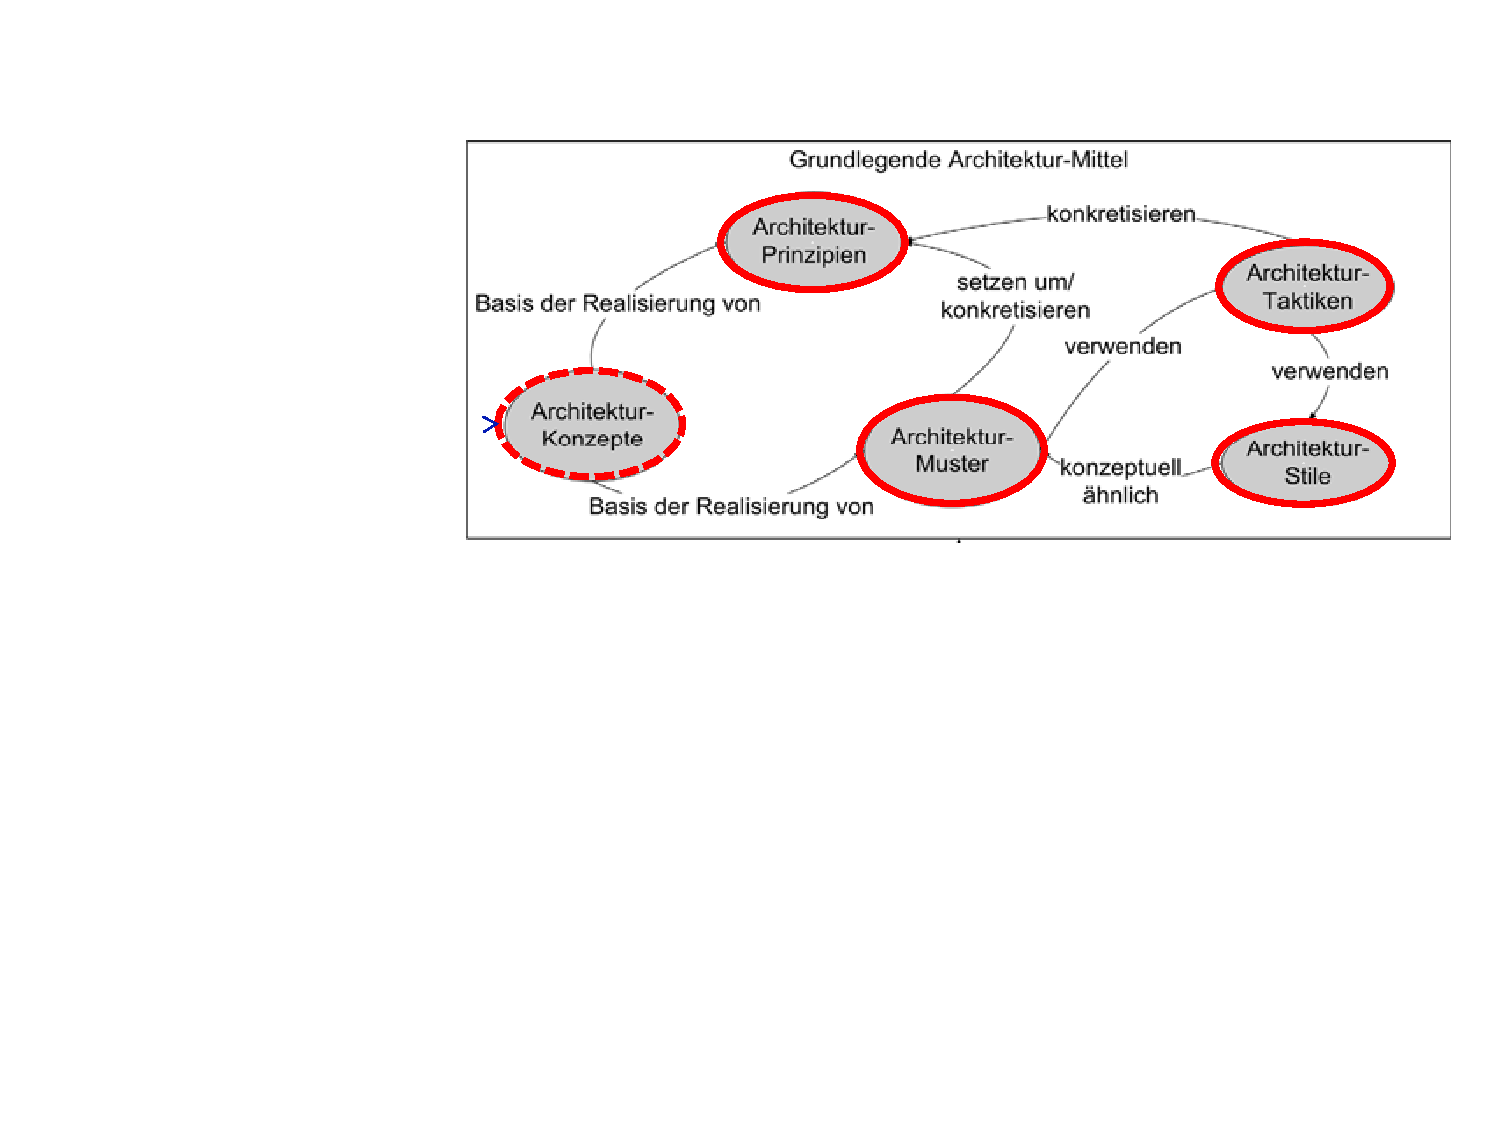
\includegraphics[width=0.7\linewidth]{fig/begriffe}
\caption{Grundlegende Begriffe}
\label{fig:begriffe}
\end{figure}

Bei einem Architekturentwurf werden Anforderungen, Qualitätsmerkmale und Rahmenbedingungen in den Prozess hineingegeben und heraus kommt eine Architektur welche durchführbar und entwicklungsfähig ist. Um so eine Architektur hinzukriegen, werden die Methoden in Abbildung \ref{fig:begriffe} angewendet. Abbildung \ref{fig:twin-peaks} zeigt das erweitere Twin Peaks Modell. Es soll aufzeigen dass die Architektur der Vermittler zwischen Anforderungen und Konstruktion ist. Zudem wird das ganze System in einem iterativen Prozess entworfen, was die Spirale darstellen soll.

\begin{figure}
\centering
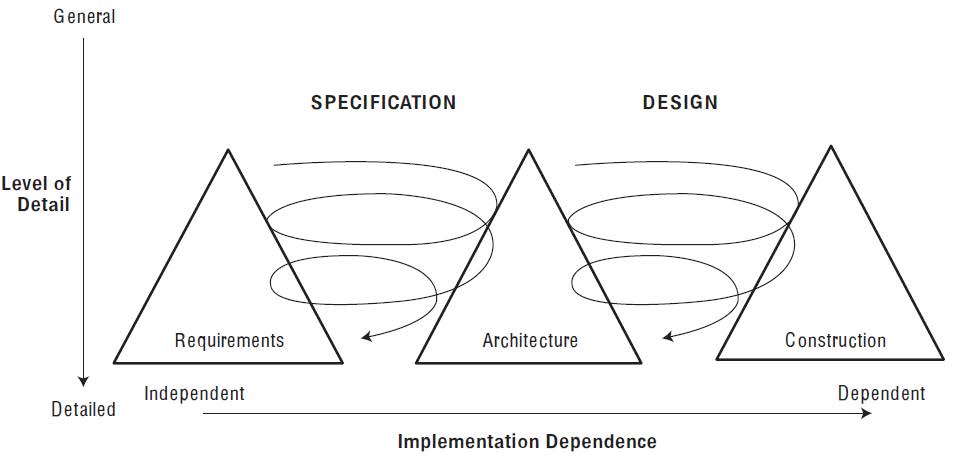
\includegraphics[width=0.7\linewidth]{fig/twin-peaks}
\caption{Erweitertes Twin Peaks Modell}
\label{fig:twin-peaks}
\end{figure}

Der iterative, inkrementelle Prozess des Architekturentwurfs läuft immer gleich ab:
\begin{enumerate}
	\item Analyse der Anforderungen und Auflösung von Konflikten
	\item Anwendung von Prinzipien, Taktiken \& Mustern
	\item Treffen von Entscheidungen \& Kompromissen
	\item Bewertung von Alternativen
	\item Bereitstellen von Sichten für Beteiligte
	\item Dokumentation und Bewertung von Entscheidungen
	\item Wenn Entwurf ok umsetzen sonst \verb|goto 1|
\end{enumerate}
Zum Schluss: Jedes System hat eine Architektur auch wenn keine Beschreibung ausserhalb des Codes existiert und sie in der Implementierung schwer zu erkennen ist.

\section{Funktionale Anforderungen: Use cases und User Stories}
\label{sec:funktionale-anforderungen}

Anforderungen müssen SMART sein. SMART bedeutet:
\begin{description}
	\item[Specific:] Eindeutig und konsistent (Beschrieben mit angemessenem Detaillierungsgrad)
	\item[Measurable:] Messbar (Wie kann beurteilt werden, ob die Anforderung erreicht wurde?)
	\item[Attainable:] Erreichbar (Technisch machbar mit dem aktuellen Stand der Technik)
	\item[Realizable:] Umsetzbar (Unter den gegebenen Randbedingungen und verfügbare Ressourcen)
	\item[Traceable:] Nachverfolgbar (Konzeption - Spezifikation - Design - Implementation - Test)
\end{description}

\section{Nichtfunktionale Anforderungen: Szenarios}

Eine Software richtet sich nicht nur nach den Anforderungen des Kunden (funktionalen Anforderungen), sondern wird auch durch Qualitätsansprüche an die Architektur (nichtfunktionale Anforderungen) beeinflusst. Nichtfunktionale Anforderungen werden einerseits durch Randbedingungen (Constraints) vorgegeben. So muss z.B. eine bestehende Softwareplattform genutzt werden oder die Zeit und Ressourcen sind zu knapp um eine verteilte Anwendung zu bauen. Die Randbedingungen schränken den Architekten bei seinen Entscheidungen also ein. 
Es gibt aber auch nichtfunktionale Anforderungen die ein Architekt sehr wohl beeinflussen kann. Dazu gehören z.B. Benutzbarkeit, Erweiterbarkeit usw. Das sind die sogenannten Qualitätsattribute. Qualitätsattribute müssen immer messbar und testbar sein. Da ein Qualitätsattribut wie eine Anforderung ist, muss auch diese SMART (siehe Abschnitt \ref{sec:funktionale-anforderungen}) sein. Die Qualitätsattribute lassen sich durch bestimmte Strukturen und Verhaltensweisen erfüllen, die von der Architektur vorgegeben werden. Funktionale Anforderungen werden erfüllt, indem bestimmte Elemente der Architektur eine Aufgabe umsetzen. Die funktionalen Anforderungen bestimmen also nicht die Architektur. 
Die Qualitätsattribute sind nicht unabhängig voneinander, weil Qualität nur indirekt messbar ist und für jeden Stakeholder etwas anderes bedeutet. Auch wenn alle funktionalen Anforderungen umgesetzt wurden, muss das nicht heissen man hat eine qualitativ hochwertige Software geschrieben. Allerdings darf man auch nicht nur auf Qualität setzen, weil dann keine Features umgesetzt werden. Deshalb sollte man immer Kompromisse bei seinen Entscheidungen eingehen.

Qualitätsattribute lassen sich in Szenarien festhalten. Ein Szenario besteht immer aus folgenden Elementen:
\begin{itemize}
	\item Quelle des Auslösers (Benutzer, Entwickler)
	\item Auslöser / Ereignis
	\item Umgebung (zur Laufzeit, während Installation)
	\item Systembestandteil (z.B GUI oder Backend)
	\item Antwort / Reaktion
	\item Antwortmetrik (Wie messen wir die Antwort?)
\end{itemize}
Ein Qualitätsattribut lässt sich problemlos in mehrere Szenarien aufschlüsseln, damit die Anforderung detaillierter beschrieben werden kann. Hat man die Szenarien bis ins Detail ausgearbeitet, können Taktiken und Muster angewendet werden um die gewünschten Ergebnisse zu erhalten.
Nachfolgend werden einige Qualitätsattribute genauer beschrieben.

\subsection{Availability}

Funktionalitäten sind vorhanden und benutzbar wenn sie gebraucht werden. Das System muss also stabil und zuverlässig sein. Ein Ausfall sollte möglichst verhindert werden. Kommt es trotzdem zu einem Ausfall muss man das System in einer bestimmten Zeit wiederherstellen. Es können folgende Fehler auftreten (Auslöser eines Szenarios):
\begin{description}
	\item[Omission:] keine Antwort auf eine Anfrage
	\item[Crash:] Omissions treten wiederholt auf
	\item[Timing:] Response tritt zu falscher Zeit ein (zu früh, zu spät)
	\item[Response:] falscher Response des Systems
\end{description}
Diese Fehler können folgendermassen bekämpft werden:
\begin{description}
	\item[Prevention:] Einbau von Redundanz, Sicherheitsfunktionen oder Lastbegrenzungen
	\item[Detection \& Isolation:] Logging des Fehlers
	\item[Recovery:] Benachrichtigung von Benutzern und anderen Systemen, Aktionen zur Schadensbegrenzung oder einschränken der Verfügbarkeit oder Funktionalität des betroffenen Systems
\end{description}
Folgende Messwerte können zur Statistik verwendet werden:
\begin{itemize}
	\item Mean Time to Recover (MTTR)
	\item Mean Time to Failure (MTTF)
	\item Mean Time between Failure (MTBF)
\end{itemize}
\begin{figure}[h!]
\centering
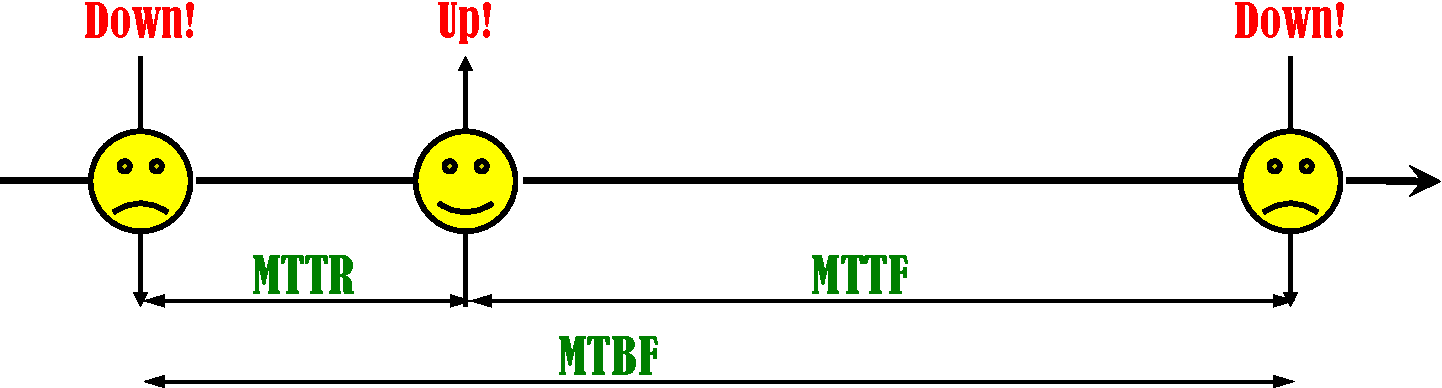
\includegraphics[width=\linewidth]{fig/mbegriffe}
\caption{M-Begriffe}
\label{fig:mbegriffe}
\end{figure}

\subsection{Interoperability}

Die Interoperabilität beschreibt den Grad in dem zwei oder mehr Systeme Information sinnvoll austauschen können. Dabei geht es um die Schnittstellen mit anderen Systemen und wie diese Systeme die Daten interpretieren.

\subsection{Modifiability}

Die Modifizierbarkeit beschreibt welche Ressourcen für eine Änderung notwendig sind und wie hoch das Risiko dafür ist. Abbildung \ref{fig:modifiability} zeigt ein Beispiel-Szenario für die Erweiterbarkeit.

\begin{figure}[h!]
\centering
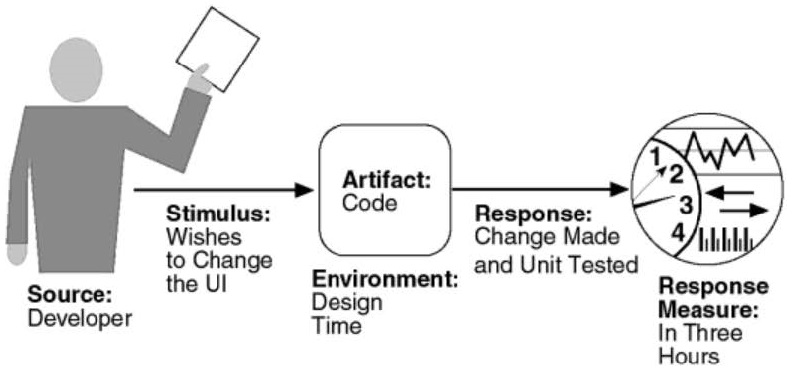
\includegraphics[width=0.7\linewidth]{fig/modifiability}
\caption{Szenario Modifiability}
\label{fig:modifiability}
\end{figure}

\subsection{Performance}

Die Performance beschreibt die Zeit in der ein System auf ein bestimmtes Ereignis reagiert. Messwerte sind Latenz (Zeit zwischen Ereignis und Reaktion), Durchsatz oder Jitter (Anzahl nicht verarbeiteter Events).

\begin{figure}[h!]
\centering
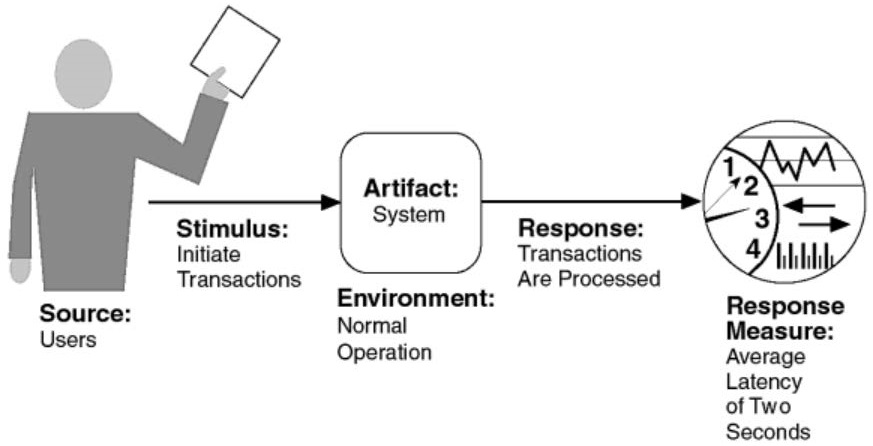
\includegraphics[width=0.7\linewidth]{fig/performance}
\caption{Szenario Performance}
\label{fig:performance}
\end{figure}

\subsection{Security}

Ein System soll Informationen vor nicht berechtigtem Zugriff schützen. Auch die Integrität der Daten muss gewährleistet sein. Darum müssen Angriffe erkannt und entsprechend darauf reagiert werden. Abbildung \ref{fig:security} zeigt ein mögliches Szenario.

\begin{figure}[h!]
\centering
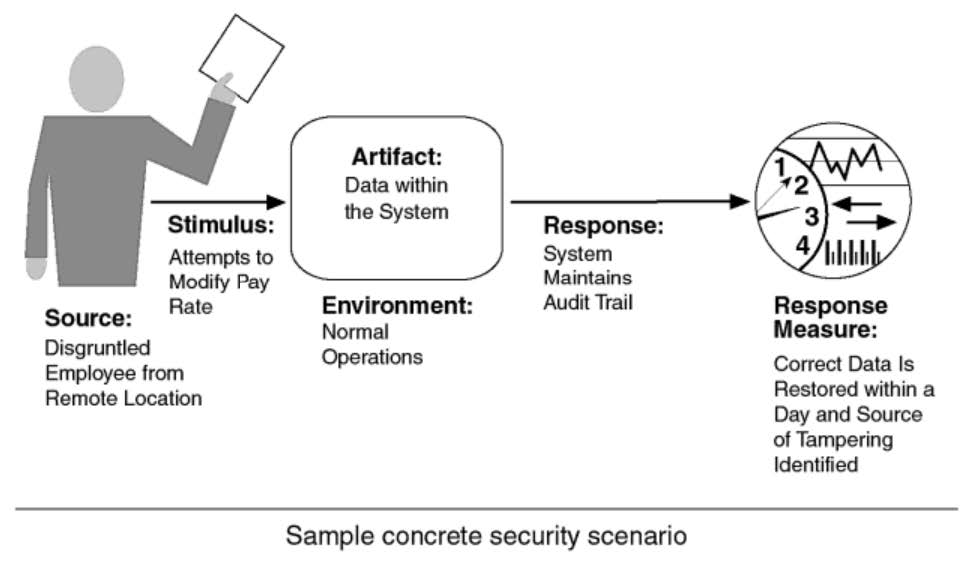
\includegraphics[width=0.7\linewidth]{fig/security}
\caption{Szenario Security}
\label{fig:security}
\end{figure}

\subsection{Testability}

Die Testbarkeit ist die Einfachheit mit der Fehler im System festgestellt werden können. Abbildung \ref{fig:testability} zeigt ein mögliches Szenario.

\begin{figure}[h!]
\centering
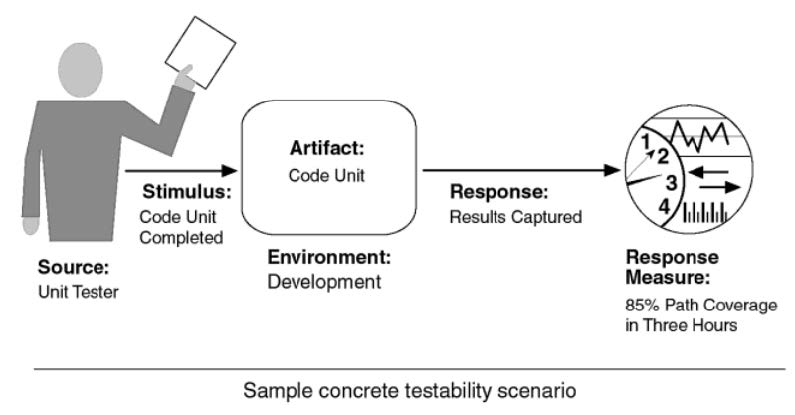
\includegraphics[width=0.7\linewidth]{fig/testability}
\caption{Szenario Testability}
\label{fig:testability}
\end{figure}

\subsection{Usability}

Mit Usability ist die Benutzerfreundlichkeit eines Systems gemeint. So soll z.B. die Einarbeitung in ein neues System nicht viel Zeit in Anspruch nehmen. Abbildung \ref{fig:usability} zeigt ein mögliches Szenario.

\begin{figure}[h!]
\centering
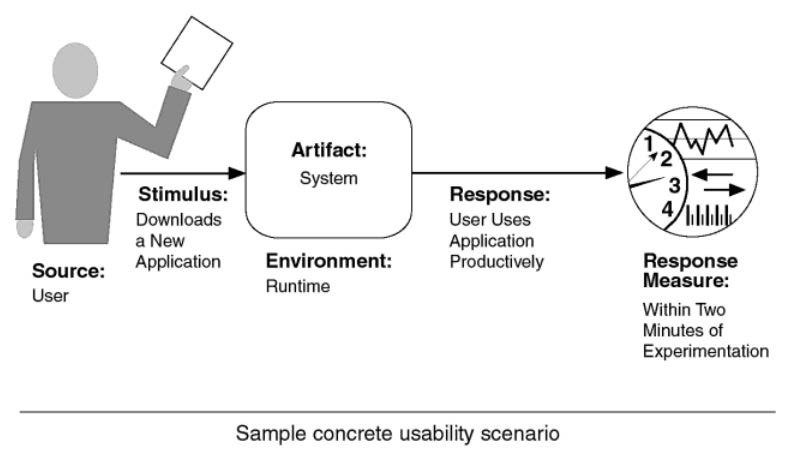
\includegraphics[width=0.7\linewidth]{fig/usability}
\caption{Szenario Usability}
\label{fig:usability}
\end{figure}


\section{Prinzipien \& Taktiken}

\section{Stile und Muster}

\section{Sichten, Architekturentscheidungen und Dokumentation}

\section{Bewertung von Architekturen (ATAM)}

\section{Beruf des IT Architekten}

\section{Fallstudie Fillialbestellsystem aus Modul Applikationsentwicklung}